
\medskip

Un sac contient 20 jetons qui sont soit jaunes, soit verts, soit rouges, soit bleus. On considère l'expérience suivante : tirer au hasard un jeton, noter sa couleur et remettre le jeton dans le sac. Chaque jeton a la même probabilité d'être tiré. 

\medskip

\begin{enumerate}
\item Le professeur, qui connaît la composition du sac, a simulé un grand nombre de fois l'expérience avec un tableur. Il a représenté ci-dessous la fréquence d'apparition des différentes couleurs après \np{1000} tirages. 

%\begin{center}
%\begin{tabularx}{\linewidth}{|l|*{4}{>{\centering \arraybackslash}X|}}\hline
%Couleur&jaune&vert&rouge&bleu\\ \hline
%Fréquence d'apparition&0,5&0,25&0,2&0,05\\ \hline
%\end{tabularx}
%\end{center} 

\begin{center}
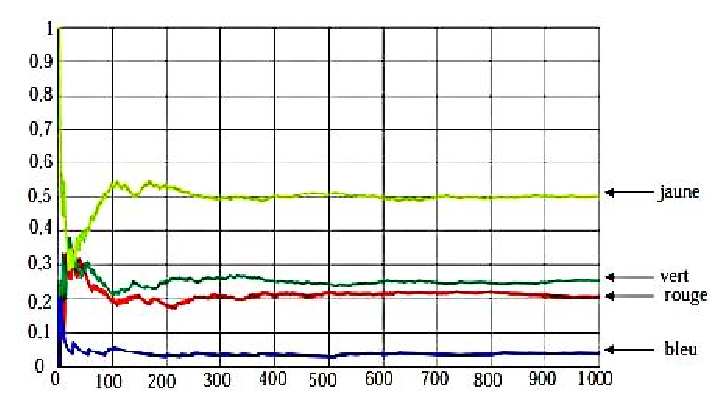
\includegraphics[width=10cm]{jetons.eps}
\end{center}

\begin{enumerate}
\item Quelle couleur est la plus présente dans le sac ? Aucune justification n'est attendue. 
\item  Le professeur a construit la feuille de calcul suivante :

\begin{center}
\begin{tabularx}{0.9\linewidth}{|c|*{3}{>{\centering \arraybackslash}X|}}\hline 
&A&     B&     C\\ \hline   
1&   Nombre de   tirages&   Nombre de fois où  un jeton rouge est  apparu&Fréquence   d'apparition de la   couleur rouge\\ \hline   
2 	&  1	&  0&   0\\ \hline   
3  	&  2	&  0&   0\\ \hline   
4  	&  3 	&  0&   0\\ \hline   
5   & 4		&  0&   0 \\ \hline  
6   &  5	&  0&   0\\ \hline   
7   &  6	&  1&   \np{0,166666667}\\ \hline   
8   &  7	&  1&   \np{0,142857143}\\ \hline 
9   &  8 	&  1&   0,125 \\ \hline  
10 	&  9	&  1&   \np{0,111111111}\\ \hline   
11 	&  10	&  1&   0,1 \\ \hline
\end{tabularx}
\end{center} 

Quelle formule a-t-il saisie dans la cellule C2 avant de la recopier vers le bas ?
\end{enumerate}
\item On sait que la probabilité de tirer un jeton rouge est de $\dfrac{1}{5}$.  

Combien y a-t-il de jetons rouges dans ce sac? 
\end{enumerate}

\vspace{0,5cm} 

